\documentclass[11pt,a4paper]{article}

% ============================================================
% Packages
% ============================================================
\usepackage[utf8]{inputenc}
\usepackage[T1]{fontenc}
\usepackage{amsmath,amssymb,amsthm}
\usepackage{booktabs}
\usepackage{geometry}
\usepackage{enumitem}
\usepackage{graphicx}
\usepackage{hyperref}
\usepackage{xcolor}
\usepackage{tikz}
\usetikzlibrary{shapes.geometric, arrows.meta, positioning, fit, calc}
\usepackage{algorithm}
\usepackage{algorithmic}
\usepackage{multirow}
\usepackage{caption}
\usepackage{subcaption}
\usepackage{float}
\usepackage{tcolorbox}

\geometry{margin=1in}

\hypersetup{
    colorlinks=true,
    linkcolor=blue!60!black,
    citecolor=green!50!black,
    urlcolor=blue!70!black
}

% ============================================================
% Custom commands
% ============================================================
\newcommand{\stage}[1]{\textbf{Stage #1}}
\newcommand{\RR}{\mathbb{R}}
\newcommand{\bx}{\mathbf{x}}
\newcommand{\clip}{\mathrm{clip}}
\newcommand{\sigmoid}{\sigma}
\newcommand{\opnorm}[1]{\mathrm{norm}(#1)}

\definecolor{stagecolor}{RGB}{30,80,150}
\definecolor{inputcolor}{RGB}{0,120,60}
\definecolor{outputcolor}{RGB}{180,50,30}
\definecolor{notecolor}{RGB}{120,80,0}
\definecolor{newcolor}{RGB}{180,0,120}

\newtcolorbox{stagebox}[1]{
    colback=blue!3, colframe=stagecolor, fonttitle=\bfseries\large,
    title={#1}, arc=2mm, boxrule=0.8pt
}

\newtcolorbox{iobox}{
    colback=gray!5, colframe=gray!50, arc=1mm, boxrule=0.5pt, left=4pt, right=4pt, top=3pt, bottom=3pt
}

\newtcolorbox{newstagebox}[1]{
    colback=red!2, colframe=newcolor, fonttitle=\bfseries,
    title={#1}, arc=2mm, boxrule=0.8pt
}

% ============================================================
\title{\textbf{ProveTok v3.0: Token-Gated Evidence Routing\\for Grounded 3D CT Report Generation}\\[6pt]
\large Internal Proposal --- Execution Spec \& Experiment Plan}
\author{ProveTok Team}
\date{Last update: 2026-03-21}

\begin{document}
\maketitle
\tableofcontents
\newpage

% ============================================================
\section{Scope and Claim Boundary}

% ============================================================

\subsection{What We Do}
We study 3D CT report generation with \textbf{sentence-level evidence commitment} via \textbf{token-gated generation}.
A frozen 3D encoder is run once to construct a per-volume token bank of $B$ spatial evidence tokens (each with a 3D bbox + feature), and \emph{all} sentences route from this same bank.
Each sentence is generated with only a small routed subset of $k\ll B$ tokens, and the routed token IDs become the sentence citations --- turning evidence into a \emph{hard interface}.

\paragraph{Report format (fixed in matched-compute comparisons).}
We generate a report as a sequence of $L$ sentences.
In all matched-compute experiments, $L$ is \,\textbf{held fixed} (either the reference sentence count under teacher forcing, or the output of a frozen planning policy) and is \,\emph{not} tuned as a compute-matching knob.


\subsection{Core Claims (Oral-Ready)}
\begin{itemize}[nosep]
\item \textbf{C1 (Main thesis): Evidence \emph{commitment} interface.}
Turn evidence from \emph{available} to \emph{mandatory}: every sentence must \emph{commit} to $k$ localized tokens drawn from a fixed token bank, and these token IDs are emitted as citations.
At matched LLM-token compute and fixed sentence count $L$, this commitment interface yields substantially higher \emph{audited faithfulness} than global-prefix baselines.
\item \textbf{C2 (Enabler): Token-gated generation + lightweight router.}
A minimal router (a single projection matrix) trained from report sentences and coarse weak labels is sufficient to select useful evidence at low overhead; gating ensures the sentence can use \emph{only} the routed tokens.
\item \textbf{C3 (Validation): Deterministic audit + counterfactuals.}
We pair the interface with deterministic verifier rules and factorial counterfactuals (``wrong location'' vs.\ ``wrong content'') that directly test evidence use, and report verifier pass rate and counterfactual sensitivity alongside standard text metrics.
\end{itemize}

\noindent\textbf{Note.}
Our core claim is that sentence-level commitment (gating) improves \emph{audited faithfulness} at matched compute and fixed $L$, compared with global-prefix baselines where evidence is optional.


\subsection{One-Minute Oral Narrative (Story in 6 Sentences)}
\begin{tcolorbox}[colback=blue!2, colframe=stagecolor, arc=1mm, boxrule=0.5pt, left=6pt, right=6pt, top=4pt, bottom=4pt]
\small
\begin{enumerate}[nosep]
    \item \textbf{Problem:} 3D CT report generators can score well yet remain untrustworthy because evidence is not \emph{explicitly bound} to each sentence.
    \item \textbf{Observation / question:} with a single global visual prefix, evidence is optional; the model may ignore the visual channel entirely, so faithfulness cannot be audited.
    \item \textbf{Key idea:} replace the global prefix with \textbf{per-sentence top-$k$ token gating} so each sentence conditions on a small, localized evidence set.
    \item \textbf{By construction:} the routed token IDs are the sentence citations (no post-hoc attribution), making the evidence channel externally auditable.
    \item \textbf{Rigorous tests:} we evaluate under matched compute (tokens + a quadratic attention proxy), deterministic verifier rules, and targeted counterfactuals that disentangle ``wrong location'' from ``wrong content''.
    \item \textbf{Takeaway:} we will show that report-level text metrics can change little while verifier pass rate and counterfactual sensitivity change dramatically---suggesting the field needs evaluation paradigms that test evidence use, not just text similarity.
\end{enumerate}
\end{tcolorbox}


\subsection{Supporting Components (Engineering, Not Primary Novelty)}
\begin{itemize}[nosep]
    \item \textbf{Token bank construction} (adaptive split, artifact gating, boundary caching) --- an efficient way to produce $B$ spatial tokens from frozen features.
    \item \textbf{Multi-granularity generation} (overview-to-detail) --- enabled by constraining routing depth; presented as qualitative capability rather than a central claim.
\end{itemize}

\subsection{What We Do NOT Claim}
\begin{itemize}[nosep]
    \item Universal cross-domain transfer beyond chest CT.
    \item Structural modification to the LLM (no cross-attention injection; no architecture changes). We serialize 3D evidence as a structured text prompt (evidence card) and use the standard text interface; we do \emph{not} inject visual embeddings into the LLM hidden states.
    \item Fully end-to-end joint training of encoder + split + router + LLM.
    \item Pixel-perfect (segmentation-level) anatomy grounding; atlas supervision is coarse by design.
\end{itemize}

% ============================================================

\section{Architecture Contract (Frozen)}
% ============================================================

\subsection{Encoder (Frozen)}
Visual encoder family is frozen: default is a frozen SwinUNETR 3D encoder (pretrained on BTCV).
The encoder produces a dense feature volume $F \in \RR^{C \times D' \times H' \times W'}$ with $C{=}768$ channels from a $128^3$ input volume.
No encoder-family swap in main experiments.

\textbf{Why frozen --- three reasons:}

\emph{(i) Ablation fairness.}
If the encoder is fine-tuned jointly with the split strategy or routing module, performance changes cannot be attributed to a single component. Freezing the encoder ensures all experiments (adaptive vs.\ uniform, prefix vs.\ gated, different $k$) operate on the \emph{same} feature space, keeping ablation variables strictly isolated.

\emph{(ii) Computational feasibility.}
With 1--2 A100 GPUs and a 30-day timeline, fine-tuning a 3D SwinUNETR on full CT volumes would consume 3--5 days per run. Freezing the encoder reduces it to a single forward pass; feature maps are cached to disk and reused across all subsequent experiments, accelerating iteration by an order of magnitude.

\emph{(iii) Compatibility with pretrained encoders.}
Existing 3D medical vision encoders (CT-CLIP, Med3D, SwinUNETR pretrained on BTCV) carry rich pretrained representations. Freezing preserves these representations without risking catastrophic forgetting or requiring task-specific fine-tuning. If the encoder were fine-tuned, the feature distribution would shift, invalidating the split scoring statistics ($H_i$, $P_i$, $B_i$) and requiring re-calibration of all hyperparameters.

Joint encoder--split optimization is deferred to future work.

\subsection{Pipeline Insertion}
\begin{align*}
&\text{Volume} \;\to\; \text{Frozen 3D Encoder} \;\to\; F \;\to\; \text{Adaptive Split} \;\to\; \text{Top-}B\text{ Tokens}\\
&\quad\to\; \underbrace{\text{Router} \;\to\; \text{Evidence Card} \;\to\; \text{Gated LLM}}_{\text{per-sentence}} \;\to\; \text{Report}
\end{align*}

\subsection{Token Contract}
Each exported token carries:
\[
(\texttt{token\_id},\; \texttt{bbox\_3d},\; \texttt{center},\; \texttt{level},\; \mathbf{f}_i^{\mathrm{export}} \in \RR^{768},\; \texttt{score},\; \texttt{split\_source}\; [\texttt{, anatomy\_label}])
\]

% ============================================================
\section{Complete Workflow (Seven Stages)}
\label{sec:workflow}
% ============================================================

\paragraph{Narrative focus (oral).}
Stage~3 (token-gated generation) is the core contribution and the main oral narrative.
Stages~0--2 (token-bank construction) and Stages~4--5 (verification/re-routing) are supporting components; in an oral-length paper we would summarize them in the main text and place full implementation details in the appendix.

\begin{figure}[H]
\centering
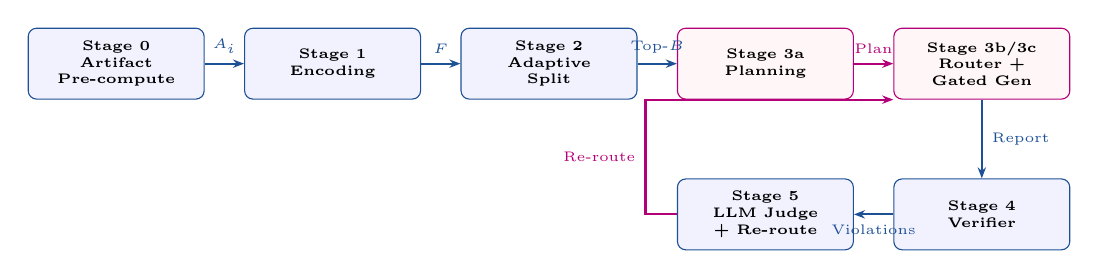
\begin{tikzpicture}[
    node distance=0.4cm and 0.5cm,
    block/.style={rectangle, draw=stagecolor, fill=blue!5, rounded corners=3pt,
                  text width=2.0cm, minimum height=0.9cm, align=center, font=\tiny\bfseries},
    newblock/.style={rectangle, draw=newcolor, fill=red!3, rounded corners=3pt,
                  text width=2.0cm, minimum height=0.9cm, align=center, font=\tiny\bfseries},
    arr/.style={-{Stealth[length=4pt]}, thick, stagecolor},
    newarr/.style={-{Stealth[length=4pt]}, thick, newcolor}
]
\node[block] (s0) {Stage 0\\Artifact\\Pre-compute};
\node[block, right=of s0] (s1) {Stage 1\\Encoding};
\node[block, right=of s1] (s2) {Stage 2\\Adaptive\\Split};
\node[newblock, right=of s2] (s3a) {Stage 3a\\Planning};
\node[newblock, right=of s3a] (s3b) {Stage 3b/3c\\Router +\\Gated Gen};
\node[block, below=1.0cm of s3b] (s4) {Stage 4\\Verifier};
\node[block, left=of s4] (s5) {Stage 5\\LLM Judge\\+ Re-route};

\draw[arr] (s0) -- node[above, font=\tiny]{$A_i$} (s1);
\draw[arr] (s1) -- node[above, font=\tiny]{$F$} (s2);
\draw[arr] (s2) -- node[above, font=\tiny]{Top-$B$} (s3a);
\draw[newarr] (s3a) -- node[above, font=\tiny]{Plan} (s3b);
\draw[arr] (s3b) -- node[right, font=\tiny]{Report} (s4);
\draw[arr] (s4) -- node[below, font=\tiny]{Violations} (s5);
\draw[newarr] (s5.west) -- +(-0.4,0) |- node[left, font=\tiny, pos=0.25]{Re-route} (s3b.south west);
\end{tikzpicture}
\caption{ProveTok v3.0 pipeline. \textcolor{newcolor}{Pink boxes} are new in v3.0 (token-gated generation).}
\label{fig:pipeline}
\end{figure}

% ============================================================
% STAGE 0--2: UNCHANGED FROM v2.5
% ============================================================

\subsection{Stages 0--2: Deterministic Token Bank Construction (Summary; details in Appendix~\ref{app:stage0-2})}

\begin{stagebox}{Stages 0--2 --- Deterministic Token Bank}
\textcolor{inputcolor}{\textbf{Input:}} Raw CT volume $V \in \RR^{D\times H\times W}$.\\
\textcolor{outputcolor}{\textbf{Output:}} A bank of at most $B$ evidence tokens $\{\tau_i\}_{i=1}^{|\mathcal{C}|}$ with \emph{stable IDs}, multiscale geometry (octree level $\ell_i$, voxel/mm bboxes), pooled visual features $\mathbf{f}_i \in \RR^{768}$, and cached boundary context for clean crop semantics.
\end{stagebox}

\paragraph{Stage 0: voxel-space artifacts.}
We deterministically pre-compute a small set of voxel-space artifacts (e.g., gradient magnitude, simple organ masks, and boundary cues) used \emph{only} to score split candidates.
These artifacts do not depend on learned parameters and are cached on disk.

\paragraph{Stage 1: one-shot frozen encoding.}
We run a frozen SwinUNETR 3D encoder once per volume to obtain a dense feature volume $F \in \RR^{768 \times D' \times H' \times W'}$.
All downstream tokenization and routing operate on these frozen features; no encoder fine-tuning is used in our core claims.

\paragraph{Stage 2: adaptive octree split.}
Starting from a coarse grid ($d_0{=}2$, giving $4^3{=}64$ initial cells on a $128^3$ volume), we iteratively score cells by a fixed, deterministic rule (uncertainty + boundary + optional semantic prior) and split the highest-scored cells until reaching the token bank size $B$ (or max depth $d_{\max}{=}5$).
Each leaf cell is exported as an evidence token with a stable reference, geometry, and pooled feature $\mathbf{f}_i$; we additionally cache a small boundary blend (parameter $\beta{=}0.1$) so tokens retain minimal neighbor context.
\textbf{All implementation details (soft gate, uncertainty branch, quantile normalization, overlap margin, boundary caching, and export format) are moved to Appendix~\ref{app:stage0-2} to preserve oral-friendly pacing.}

\subsection{Stage 3: Token-Gated Generation (v3.0 Core Contribution)}
\label{sec:gated_gen}

\begin{newstagebox}{Stage 3 --- Token-Gated Generation (NEW in v3.0)}
\textcolor{inputcolor}{\textbf{Input:}} Top-$B$ evidence tokens (features $\mathbf{f}_i \in \RR^{768}$ + bboxes + metadata); LLM (Llama-3.1-8B-Instruct).\\
\textcolor{outputcolor}{\textbf{Output:}} Report text with \textbf{auditable per-sentence citations}.

\textbf{Key idea:} replace a single global visual prefix with \emph{per-sentence} top-$k$ \textbf{token gating}.
The routed token IDs are the sentence citations \emph{by construction} (no post-hoc extraction).
\end{newstagebox}

\subsubsection{Motivation: ``Evidence Optional'' in Global-Prefix LLMs}
In a standard visual-prefix setup, all $B$ tokens are prepended to the prompt.
Evidence becomes \emph{available} but not \emph{mandatory}: the model can generate plausible text while largely ignoring the visual channel, and post-hoc citations can therefore be broad or inconsistent.

Token-gated generation turns evidence usage into a \emph{hard interface}:
for each sentence, only a small routed subset of $k$ tokens enters the prompt, which forces every sentence to be conditioned on explicit spatial evidence.

\subsubsection{Phase 1: Rule-Based Sentence Planning}
\label{sec:planning}

\begin{iobox}
\textcolor{inputcolor}{\textbf{Input:}} Reference report text (or planned findings).\\
\textcolor{outputcolor}{\textbf{Output:}} Ordered list of \texttt{SentencePlan} objects, each containing: sentence topic, anatomy keyword (if matched), expected octree level range, expected volume range, and negation flag.
\end{iobox}

\paragraph{Deterministic extraction.}
Planning is implemented as a \textbf{rule-based} module (not an LLM call).
The reference report is split into sentences by punctuation/newlines (up to $L_{\max}{=}8$ sentences), and each sentence is processed by three deterministic extractors:

\begin{enumerate}[nosep]
    \item \textbf{Anatomy keyword extraction:} regex search against a fixed anatomy lexicon (e.g., ``right lung'', ``left lower lobe'', ``mediastinum'', ``bilateral''). Matched keywords are mapped to coarse 3D bounding boxes via a predefined atlas. If no keyword is matched, $\mathrm{bbox}_{\mathrm{anatomy}} = \varnothing$.

    \item \textbf{Expected level range:} heuristic rules map finding descriptors to octree depth ranges:
    \begin{itemize}[nosep]
        \item Diffuse/bilateral findings (e.g., ``effusion'', ``edema'') $\to$ coarse levels $(0, 2)$
        \item Focal findings (e.g., ``nodule'', ``mass'', ``lesion'') $\to$ fine levels $(2, 5)$
        \item Unmatched $\to$ unconstrained (\texttt{None})
    \end{itemize}

    \item \textbf{Negation detection:} lexicon-based check for negation words (``no'', ``without'', ``not'', ``negative for'', ``absence of'').
\end{enumerate}

\paragraph{Why rule-based planning.}
Using deterministic extraction (rather than an LLM planning call) ensures that: (i)~no additional LLM compute is consumed, (ii)~planning is exactly reproducible, and (iii)~ablation studies can isolate gating from planning quality.

\subsubsection{Phase 2: Lightweight Router}
\label{sec:router}

\begin{iobox}
\textcolor{inputcolor}{\textbf{Input:}} One sentence topic $s$; token bank $\{\mathbf{f}_i \in \RR^{d_v}\}_{i=1}^B$ ($d_v{=}768$); optional anatomy bbox.\\
\textcolor{outputcolor}{\textbf{Output:}} Routing scores $\hat{r}_i^{(s)}$ for all tokens; top-$k$ most relevant token indices.
\end{iobox}

\paragraph{Step 1: Text query encoding.}
The sentence topic $s$ is encoded by a frozen text encoder (sentence-transformers/all-MiniLM-L6-v2) into a query vector and L2-normalized:
\begin{equation}
\mathbf{q}_s = \frac{\mathrm{TextEnc}(s)}{\lVert \mathrm{TextEnc}(s) \rVert_2}, \quad \mathbf{q}_s \in \RR^{d_t}, \quad d_t = 384.
\label{eq:query}
\end{equation}

\paragraph{Step 2: Visual token projection.}
Each token's visual feature $\mathbf{f}_i \in \RR^{d_v}$ is projected into the text embedding space and L2-normalized:
\begin{equation}
\mathbf{v}_i = \frac{W_{\mathrm{proj}} \, \mathbf{f}_i}{\lVert W_{\mathrm{proj}} \, \mathbf{f}_i\rVert_2}, \quad \mathbf{v}_i \in \RR^{d_t}, \quad \lVert \mathbf{v}_i \rVert_2 = 1,
\label{eq:projection}
\end{equation}
where $W_{\mathrm{proj}} \in \RR^{d_t \times d_v}$ ($384 \times 768$) is the only learnable parameter. When $W_{\mathrm{proj}}$ is untrained, it defaults to the identity prefix $[I_{d_t} \mid \mathbf{0}]$ (first $d_t$ rows of $I_{d_v}$).

\paragraph{Step 3: Cosine routing score.}
Since both $\mathbf{q}_s$ and $\mathbf{v}_i$ are unit-normalized, the routing score is a dot product (= cosine similarity):
\begin{equation}
r_i^{(s)} = \mathbf{q}_s^\top \mathbf{v}_i = \cos(\mathbf{q}_s, \mathbf{v}_i) \in [-1, 1].
\label{eq:routing_score}
\end{equation}

\paragraph{Step 4: Spatial prior augmentation.}
If the plan provides an anatomy keyword with a corresponding atlas bbox $\mathrm{bbox}_{\mathrm{anatomy}}^{(s)}$, the routing score is augmented with a spatial IoU bonus.
We implement \textbf{two routing modes}:

\begin{itemize}[nosep]
\item \textbf{Standard mode (semantic-primary):}
\begin{equation}
\hat{r}_i^{(s)} = r_i^{(s)} + \lambda_{\mathrm{spatial}} \cdot \mathrm{IoU}(\mathrm{bbox}_i, \, \mathrm{bbox}_{\mathrm{anatomy}}^{(s)}),
\label{eq:spatial_routing}
\end{equation}
where $\lambda_{\mathrm{spatial}} = 0.3$ (default). This mode is suitable when $W_{\mathrm{proj}}$ has been trained and the semantic score $r_i^{(s)}$ is reliable.

\item \textbf{Anatomy-primary mode (for untrained $W_{\mathrm{proj}}$):}
When $W_{\mathrm{proj}}$ has not been trained via InfoNCE, the cosine score $r_i^{(s)}$ is unreliable (the visual and text embedding spaces are not aligned).
In this case, we invert the weighting so that spatial IoU dominates:
\begin{equation}
\hat{r}_i^{(s)} = \mathrm{IoU}(\mathrm{bbox}_i, \, \mathrm{bbox}_{\mathrm{anatomy}}^{(s)}) + \epsilon \cdot r_i^{(s)},
\label{eq:anatomy_primary}
\end{equation}
where $\epsilon \ll 1$ (default $\epsilon = 0.05$) makes the semantic score a tiebreaker among tokens with equal IoU.
This is the \textbf{default mode in our main experiments} (B2'v2 configuration), using IoU as the only calibrated spatial signal.
\end{itemize}

If no anatomy keyword is matched ($\mathrm{bbox}_{\mathrm{anatomy}} = \varnothing$), the spatial prior is dropped and $\hat{r}_i^{(s)} = r_i^{(s)}$.

\paragraph{Step 5: Top-$k$ selection.}
The $k$ tokens with the highest $\hat{r}_i^{(s)}$ are selected as the evidence set $E_s$ for sentence $s$ (default $k{=}8$, ties broken by token ID):
\begin{equation}
E_s = \operatorname{argtop\text{-}k}\bigl\{\hat{r}_i^{(s)} \mid i \in \{1,\ldots,B\}\bigr\}.
\label{eq:topk}
\end{equation}

\subsubsection{Phase 3: Evidence Card Construction}
\label{sec:evidence_card}

\begin{iobox}
\textcolor{inputcolor}{\textbf{Input:}} $k$ routed tokens (bboxes, levels, features); volume midline $x_{\mathrm{mid}}$; expected level range.\\
\textcolor{outputcolor}{\textbf{Output:}} Structured \texttt{EvidenceCard} summarizing spatial properties + generation constraints.
\end{iobox}

Before generation, the routed tokens are analyzed to construct an \textbf{Evidence Card} --- a structured summary that constrains what the LLM may claim about laterality and depth.
The Evidence Card computes:

\begin{enumerate}[nosep]
\item \textbf{Laterality distribution:} Each token is classified as \emph{left}, \emph{right}, or \emph{cross} based on its bbox center $x_c = (x_{\min} + x_{\max})/2$ relative to the volume midline $x_{\mathrm{mid}}$:
\[
\mathrm{side}(i) = \begin{cases}
\text{``left''} & \text{if } x_c > x_{\mathrm{mid}} + \delta \\
\text{``right''} & \text{if } x_c < x_{\mathrm{mid}} - \delta \\
\text{``cross''} & \text{otherwise}
\end{cases}
\]
where $\delta$ is the lateral tolerance (default $\delta{=}0$).

\item \textbf{Dominant side determination:}
Let $n_L, n_R, n_C$ be the counts of left, right, and cross tokens.
The dominant side is determined by the same-side ratio $\rho = \max(n_L, n_R) / (n_L + n_R)$.

\item \textbf{Laterality gate (strict mode):} Under the \texttt{strict\_laterality} flag (used in main experiments), the allowed laterality claim is determined by:
\begin{itemize}[nosep]
    \item If fewer than 2 non-cross tokens $\to$ \texttt{laterality\_allowed = none}
    \item If $\rho \ge 0.9$ and dominant count $\ge 2$ $\to$ \texttt{laterality\_allowed = left/right}
    \item If both sides have $\ge 2$ tokens $\to$ \texttt{laterality\_allowed = bilateral}
    \item Otherwise $\to$ \texttt{laterality\_allowed = none}
\end{itemize}

\item \textbf{Depth gate:} If an expected level range $[\ell_{\min}, \ell_{\max}]$ is provided, the card reports ``in\_range'' if ${\ge}75\%$ of tokens fall within the range; ``none'' otherwise.
\end{enumerate}

\paragraph{Strict-mode token cleanup.}
When \texttt{strict\_laterality} is enabled, opposite-side tokens are removed from the citation set before generation (keeping $\ge 2$ tokens). Similarly, out-of-range depth tokens may be pruned. The Evidence Card is then rebuilt on the cleaned set.

\subsubsection{Phase 4: Per-Sentence Gated Generation (Stage 3c)}
\label{sec:per_sent_gen}

\begin{iobox}
\textcolor{inputcolor}{\textbf{Input:}} Routed $k$ tokens + Evidence Card constraints + sentence topic + previously generated text (history).\\
\textcolor{outputcolor}{\textbf{Output:}} One report sentence + citations (= routed token IDs).
\end{iobox}

\paragraph{Text-based evidence interface.}
Unlike visual-prefix methods that inject token embeddings into the LLM's hidden state, we serialize the routed evidence as a \textbf{structured text prompt}.
For each planned sentence:
\begin{enumerate}[nosep]
    \item Router selects top-$k$ tokens (Phase~2).
    \item An Evidence Card is constructed (Phase~3) summarizing spatial constraints.
    \item The LLM prompt is assembled from:
    \begin{itemize}[nosep]
        \item \textbf{System message:} ``You are an expert radiologist. Generate one sentence describing the finding based on the evidence tokens provided.''
        \item \textbf{Token block:} For each routed token: token ID, octree level, center coordinates $(x,y,z)$, bbox extents, volume, and split score.
        \item \textbf{Evidence Card constraints:} \texttt{laterality\_allowed} and \texttt{depth\_allowed} fields, instructing the LLM which spatial claims are permitted.
        \item \textbf{Sentence topic:} The planned finding to describe.
        \item \textbf{History:} Previously generated sentences for coherence.
    \end{itemize}
    \item The LLM (Llama-3.1-8B-Instruct, temperature 0.3) generates one sentence.
    \item \textbf{Citation is automatic:} the routed token IDs are recorded as the citations for this sentence.
\end{enumerate}

\paragraph{Why text serialization instead of visual prefix.}
Serializing evidence as structured text allows us to: (i)~include explicit spatial constraints (Evidence Card gates) that the LLM can follow as instructions, (ii)~use any text-only LLM without architectural modifications, and (iii)~make the evidence interface fully inspectable and auditable.


\subsubsection{Compute Accounting (Matched-Compute Comparisons)}
\label{sec:compute_accounting}

We define \textbf{LLM-token compute} as the total number of tokens processed by the LLM across all forward passes:
\[
C_{\mathrm{LLM}} \;=\; \sum_{j=1}^{N_{\mathrm{calls}}} \bigl(|\mathrm{prompt}_j| + |\mathrm{gen}_j|\bigr).
\]
For token-gated generation, $N_{\mathrm{calls}}{=}L$ (one per sentence, plus optional Stage~5 re-generation for violated sentences), with $|\mathrm{prompt}_j| \approx |\mathrm{sys}| + |\mathrm{token\_block}| + |\mathrm{evidence\_card}| + |\mathrm{topic}| + |\mathrm{history}|$.


% ============================================================
\subsubsection{Projection Layer Training (InfoNCE)}
\label{sec:projection_training}

\paragraph{Training data construction (bootstrap from spatial routing).}
\textbf{Important:} $W_{\mathrm{proj}}$ training uses a \emph{bootstrap} strategy: we first run the full pipeline with the anatomy-primary routing mode (Eq.~\ref{eq:anatomy_primary}, $W_{\mathrm{proj}} = I$), which produces per-sentence citation sets guided by spatial IoU.
These citation sets serve as weak supervision for training $W_{\mathrm{proj}}$.

Concretely, from the Stage 0--4 output traces on the CT-RATE training split:
\begin{enumerate}[nosep]
    \item For each sentence $s$ in the trace, extract the text $s$ and its top-$k$ cited token IDs $\{t_1, \ldots, t_k\}$ (produced by anatomy-primary routing).
    \item Encode the sentence text to a query vector: $\mathbf{q}_s = \mathrm{TextEnc}(s) \in \RR^{d_t}$.
    \item Collect the visual features of the cited tokens: $\{\mathbf{f}_{t_1}, \ldots, \mathbf{f}_{t_k}\} \subset \RR^{d_v}$.
    \item The training pair is $(\mathbf{q}_s, \; \bar{\mathbf{f}}_s^{+})$ where $\bar{\mathbf{f}}_s^{+} = \frac{1}{k}\sum_{j=1}^k \mathbf{f}_{t_j}$ is the \textbf{mean of cited token features}.
\end{enumerate}

\paragraph{Loss function (batch contrastive InfoNCE).}
Given a batch of $N$ training pairs $\{(\mathbf{q}_n, \bar{\mathbf{f}}_n^{+})\}_{n=1}^N$, we project the positive features and compute a symmetric contrastive loss:
\begin{equation}
\mathbf{p}_n = \frac{W_{\mathrm{proj}} \, \bar{\mathbf{f}}_n^{+}}{\lVert W_{\mathrm{proj}} \, \bar{\mathbf{f}}_n^{+} \rVert_2}, \quad
\ell_{n,m} = \frac{\hat{\mathbf{q}}_n^\top \mathbf{p}_m}{\tau},
\label{eq:infonce_logits}
\end{equation}
where $\hat{\mathbf{q}}_n = \mathbf{q}_n / \lVert \mathbf{q}_n \rVert_2$ and $\tau = 0.07$ is the temperature.
The loss is:
\begin{equation}
\mathcal{L} = -\frac{1}{N} \sum_{n=1}^{N} \log \frac{\exp(\ell_{n,n})}{\sum_{m=1}^{N} \exp(\ell_{n,m})}.
\label{eq:infonce}
\end{equation}
Each query $\mathbf{q}_n$ is contrasted against its own positive projection $\mathbf{p}_n$ (numerator) versus all other queries' positive projections in the batch (in-batch negatives, denominator).

\paragraph{Interpretation.}
This loss trains $W_{\mathrm{proj}}$ so that the projected positive token mean $\mathbf{p}_n$ is close to its corresponding text query $\hat{\mathbf{q}}_n$ in cosine space, and far from other queries' projected positives.
The positives originate from the spatial routing output, so \textbf{the training signal is bootstrapped from IoU-based spatial alignment}: the projection learns to align visual features with text queries in a way that is consistent with spatial routing.

\paragraph{What is trained.}
Only $W_{\mathrm{proj}} \in \RR^{384 \times 768}$ (294,912 parameters) is trained; the text encoder (MiniLM-L6-v2) and all other components are frozen.

\paragraph{Training details.}
AdamW optimizer ($\mathrm{lr}{=}10^{-3}$, weight decay $10^{-4}$), cosine annealing, orthogonal initialization, batch size 32, up to 50 epochs with early stopping (patience 10) on validation loss.
Training runs in minutes on cached token features (no backprop through the 3D encoder).

\subsection{Stages 4--5: Verifier and LLM Judge Re-routing}
\label{sec:verifier}

\textbf{Note:} The verifier and closed-loop re-routing are \emph{auxiliary modules} that improve routing quality in practice, but are not positioned as core contributions of this work.

\begin{stagebox}{Stage 4 --- Deterministic Verifier}
\textcolor{inputcolor}{\textbf{Input:}} Generated report text + per-sentence citation mapping + token metadata (bboxes, levels).\\
\textcolor{outputcolor}{\textbf{Output:}} List of \texttt{RuleViolation}s with (rule\_id, severity, linked token IDs, message).
\end{stagebox}

\subsubsection{Verifier Contract (Deterministic and Executable)}
The verifier operates only on (i)~surface report text segmented into sentences, (ii)~the per-sentence citation list produced by routing, and (iii)~token geometry ($\texttt{bbox\_3d}$) and level ($\texttt{level}$). No model internals are used.

\paragraph{Laterality parsing (rule-based).}
We infer laterality by word-boundary-aware regex matching on a fixed lexicon:
\emph{bilateral} if the sentence contains any of \{\texttt{bilateral(ly)}, \texttt{both}\};
\emph{left} if it contains \{\texttt{left}, \texttt{lt}\} (word boundary) and not right;
\emph{right} if it contains \{\texttt{right}, \texttt{rt}\} (word boundary) and not left;
otherwise \emph{None} (laterality rules are skipped).
Word-boundary matching prevents false positives from substrings (e.g., ``hea\textbf{rt}'', ``ao\textbf{rt}a'', ``resu\textbf{lt}'').

\paragraph{Mid-sagittal plane and token side.}
The volume midline is $x_{\mathrm{mid}} = W/2$ (half the volume width in voxels).
A token's side is determined by its bbox center:
\[
\mathrm{side}(i) = \begin{cases}
\text{``left''} & \text{if } x_c > x_{\mathrm{mid}} + \delta \\
\text{``right''} & \text{if } x_c < x_{\mathrm{mid}} - \delta \\
\text{``cross''} & \text{otherwise}
\end{cases}
\]
with tolerance $\delta$ (default $\delta{=}0$).

\paragraph{Rule definitions.}
We define five per-sentence rules and two cross-sentence consistency rules:

\begin{table}[H]
\centering\small
\caption{Verifier rules. Severity values are defaults; actual severity may be scaled by gap magnitude.}
\begin{tabular}{lp{7.5cm}cc}
\toprule
Rule ID & Check & Severity & Status \\
\midrule
\textbf{R1\_LATERALITY} & If sentence claims left/right, fraction of same-side cited tokens must $\ge \rho_{\min}$ (default $\rho_{\min}{=}0.6$) & 1.0 & Active \\
\textbf{R2\_ANATOMY} & If anatomy bbox available, $\max_{i \in \mathcal{C}} \mathrm{IoU}(\mathrm{bbox}_i, \mathrm{bbox}_{\mathrm{anat}}) \ge \tau_{\mathrm{IoU}}$ (default 0.04) & 0.8 & Active \\
\textbf{R3\_DEPTH} & If expected level range $[\ell_{\min}, \ell_{\max}]$ provided, all cited tokens must satisfy $\ell_{\min} \le \ell_i \le \ell_{\max}$ & 0.7 & Active \\
\textbf{R4\_SIZE} & If expected volume range provided, union bbox volume must be in range & 0.6 & Disabled \\
\textbf{R5\_NEGATION} & Negated sentences should not cite tokens with positive-finding metadata & 1.0 & Disabled \\
\midrule
\textbf{R6a\_CROSS\_LAT} & Same anatomy keyword across sentences $\to$ no conflicting left/right claims & 0.7 & Active \\
\textbf{R6b\_CROSS\_PRES} & Same anatomy keyword $\to$ no sentence asserts presence while another asserts absence (1 violation per conflicting group) & 0.8 & Active \\
\bottomrule
\end{tabular}
\end{table}

\paragraph{Verifier configuration in main experiments.}
In the B2'v2 configuration: R4 and R5 are disabled; R1 uses $\rho_{\min}{=}0.6$ with \texttt{r1\_negation\_exempt=True} (negated sentences skip R1) and \texttt{r1\_skip\_midline=True} (midline structures exempt); R2 uses \texttt{r2\_skip\_bilateral=True} and ratio mode with $\rho_{\min}{=}0.8$.

\begin{stagebox}{Stage 5 --- LLM Judge + Action-Dispatched Re-routing}
\textcolor{inputcolor}{\textbf{Input:}} Violations from Stage~4; generated text; Evidence Cards; token scores.\\
\textcolor{outputcolor}{\textbf{Output:}} Corrected report (or de-specify fallback).
\end{stagebox}

\subsubsection{LLM Judge (Stage 5a)}
For each Stage~4 violation, an LLM judge (Llama-3.1-8B-Instruct) reviews the sentence text, violation details, and Evidence Card to produce a structured verdict:
\begin{itemize}[nosep]
    \item \texttt{confirmed}: bool --- does the violation represent a real error?
    \item \texttt{adjusted\_severity}: float --- refined severity estimate.
    \item \texttt{suggested\_action}: one of \{\texttt{drop\_laterality}, \texttt{drop\_depth}, \texttt{reroute\_same\_side}, \texttt{merge\_conflict}\}.
    \item \texttt{reasoning}: free-text explanation.
\end{itemize}
If no violation is confirmed, the sentence passes. The judge filters false positives from the deterministic verifier (e.g., cases where the verifier flags a laterality mismatch but the generated text is clinically acceptable).

\subsubsection{Action-Dispatched Repair (Stage 5b)}
For confirmed violations, repair is dispatched by the suggested action:
\begin{enumerate}[nosep]
    \item \textbf{drop\_laterality:} Strip laterality keywords (``left''/``right''/``bilateral'') from the sentence via regex. No re-routing needed.
    \item \textbf{drop\_depth:} Strip depth keywords (``upper''/``lower''/``apical''/``basal''). No re-routing needed.
    \item \textbf{reroute\_same\_side:} Filter citation set to dominant-side tokens only, re-select top-$k$ from same-side pool, regenerate with the cleaned Evidence Card.
    \item \textbf{Fallback (log-smooth penalty + regenerate):} If no specific action applies, penalize offending tokens via log-smooth reroute:
    \begin{equation}
    r_i' = r_i - \gamma \cdot \ln(1 + \mathrm{sev}_i), \quad \gamma = 2.0,
    \label{eq:log_smooth}
    \end{equation}
    re-select top-$k$ from penalized scores, and regenerate.
    \item \textbf{De-specify:} If regeneration still fails verification, strip all spatial terms from the topic and regenerate as a generic sentence (last resort).
\end{enumerate}
Maximum one correction iteration per sentence.

% ============================================================
\subsection{Stage 6: Output and Logging}

\begin{stagebox}{Stage 6 --- Output \& Logging}
\textcolor{inputcolor}{\textbf{Input:}} Final report, per-sentence routing decisions, verifier results, judge verdicts.\\
\textcolor{outputcolor}{\textbf{Output:}} Deliverable report + per-case trace log (\texttt{trace.jsonl}).
\end{stagebox}

Per-case trace log records (one JSON line per sentence):
\begin{itemize}[nosep]
    \item Per-sentence: routed token IDs, routing scores, Evidence Card, generated text, original topic.
    \item Triggered verifier rules with severity and messages.
    \item Stage~5 judge verdicts (confirmed/dismissed, suggested action, reasoning).
    \item Whether re-routing was triggered and stop reason: \texttt{no\_violation} / \texttt{drop\_laterality} / \texttt{drop\_depth} / \texttt{reroute\_same\_side} / \texttt{log\_smooth\_reroute} / \texttt{de\_specified}.
\end{itemize}

% ============================================================
\section{Hyperparameter Protocol}
\label{sec:hyperparams}
% ============================================================

\subsection{Split Parameters (unchanged from v2.5)}

\begin{table}[H]
\centering\small
\caption{Split hyperparameter search grid.}
\begin{tabular}{lll}
\toprule
Parameter & Search range & Role \\
\midrule
$\lambda_h$ & $\{0.4, 0.5, 0.6, 0.7\}$ & Uncertainty vs.\ prior \\
$\tau_A$ & $\{0.75, 0.80, 0.85, 0.90\}$ & Soft gate midpoint \\
$k_{\mathrm{gate}}$ & $\{10, 15, 20\}$ & Soft gate steepness \\
\bottomrule
\end{tabular}
\end{table}

\subsection{Router Parameters (new in v3.0)}

\begin{table}[H]
\centering\small
\caption{Router hyperparameters (defaults reflect B2'v2 configuration).}
\begin{tabular}{llll}
\toprule
Parameter & Default & Search range & Role \\
\midrule
$k$ (tokens per sentence) & 8 & $\{4, 8, 16, 32\}$ & Tokens cited per sentence \\
$\lambda_{\mathrm{spatial}}$ & 0.3 & $\{0, 0.15, 0.3, 0.5\}$ & Spatial prior strength (standard mode) \\
$\epsilon$ (tiebreak) & 0.05 & --- & Semantic tiebreaker (anatomy-primary mode) \\
$\tau_{\mathrm{IoU}}$ (routing filter) & 0.04 & $\{0.02, 0.04, 0.1\}$ & IoU threshold for spatial filter \\
$\beta$ (boundary blend) & 0.1 & $\{0, 0.05, 0.1, 0.2\}$ & Boundary context blending weight \\
$\tau$ (InfoNCE temperature) & 0.07 & $\{0.03, 0.07, 0.1, 0.2\}$ & Contrastive training temperature \\
\bottomrule
\end{tabular}
\end{table}

All parameters frozen after calibration for test evaluation.

% ============================================================
\section{Main Experiments}
\label{sec:experiments}
% ============================================================

\subsection{Datasets}

\begin{table}[H]
\centering\small
\begin{tabular}{lll}
\toprule
Dataset & Size & Purpose \\
\midrule
CT-RATE (5K subset) & 2500 train / 500 test per source & Report quality + routing diagnostics \\
RadGenome-ChestCT (5K subset) & 2500 train / 500 test per source & Spatial grounding + citation alignment \\
\bottomrule
\end{tabular}
\end{table}

\subsection{Model Variants and Ablations}

\begin{table}[H]
\centering\small
\caption{Model variants evaluated on 5K test split (500 cases, 3979 sentences).}
\begin{tabular}{lllll}
\toprule
Config & $W_{\mathrm{proj}}$ & Routing Mode & Lat.\ Filter & Purpose \\
\midrule
\textbf{B2'v2} (main) & Identity & Anatomy-primary (Eq.~\ref{eq:anatomy_primary}) & No & Main model \\
E1 (W\_proj) & Trained & Semantic rerank & No & W\_proj ablation \\
Hybrid E1 & Trained & Semantic rerank + lat.\ filter & Yes & Lat.\ filter ablation \\
\bottomrule
\end{tabular}
\end{table}

All variants share: SwinUNETR encoder (frozen), $B{=}128$ tokens, $k{=}8$, Llama-3.1-8B-Instruct (Stage 3c + Stage 5 judge), strict laterality Evidence Card v2, log-smooth reroute ($\gamma{=}2.0$, max 1 retry).


\subsection{Metrics}

\paragraph{Layer 1: Spatial Consistency (Violation Rate).}
\begin{itemize}[nosep]
    \item \textbf{Violation rate (raw):} fraction of sentences with $\ge 1$ verifier violation.
    \item \textbf{Violation rate (judge-confirmed):} fraction after LLM judge filtering.
    \item \textbf{Per-rule breakdown:} R1 (laterality), R3 (depth), R6b (cross-presence) counts.
\end{itemize}

\paragraph{Layer 2: NLG Quality.}
BLEU-4, ROUGE-L, METEOR (generated text vs.\ original topic).

\paragraph{Statistical protocol.}
Patient-level paired bootstrap (5000 resamples), 95\% CI via percentile method, Holm step-down correction for multiple comparisons.

\subsection{Main Results}

\paragraph{Comparison with published methods.}
Table~\ref{tab:main_nlg} compares ProveTok (B2'v2 configuration) with published CT report generation methods on both datasets.
Note that task formulations differ: baselines generate full reports end-to-end, while ProveTok generates sentence-level text with topic guidance.
Evaluation protocols also differ (published vs.\ our train/valid/test split), so direct comparison requires caution.

\begin{table}[H]
\centering\small
\caption{Comparison with published methods on CT-RATE and RadGenome-ChestCT.
ProveTok uses the B2'v2 configuration (Evidence Card v2 + spatial routing).
Baselines use published evaluation protocols; ProveTok uses our split (\texttt{seed=42}, 2000/250/250).
Metrics are not directly comparable due to different task formulations (full-report vs.\ sentence-level generation).}
\label{tab:main_nlg}
\begin{tabular}{@{}llc ccc@{}}
\toprule
\textbf{Dataset} & \textbf{Method} & \textbf{Protocol}
  & \textbf{BLEU-4}$\uparrow$ & \textbf{METEOR}$\uparrow$ & \textbf{ROUGE-L}$\uparrow$ \\
\midrule
CT-RATE & CT2Rep      & published & 0.172 & 0.173 & 0.243 \\
CT-RATE & CT-AGRG     & published & 0.172 & 0.196 & 0.280 \\
CT-RATE & \textbf{ProveTok (ours)} & our split & \textbf{0.467} & \textbf{0.603} & \textbf{0.626} \\
\midrule
RadGenome & MedVInT   & published & 0.246 & 0.404 & 0.326 \\
RadGenome & Reg2RG    & published & 0.249 & 0.441 & 0.367 \\
RadGenome & \textbf{ProveTok (ours)} & our split & \textbf{0.506} & \textbf{0.660} & \textbf{0.680} \\
\bottomrule
\end{tabular}
\end{table}

\paragraph{Spatial consistency results (5K test split).}
Table~\ref{tab:main_results} compares the three routing variants on the 5K test split (500 cases, 3979 sentences).

\begin{table}[H]
\centering\small
\caption{Spatial consistency and NLG results on 5K test split (500 cases, 3979 sentences). B2'v2 = official model.}
\begin{tabular}{lccc}
\toprule
& \textbf{B2'v2} (main) & E1 (W\_proj) & Hybrid E1 \\
\midrule
R1 (Laterality) $\downarrow$ & \textbf{2} & 105 & 104 \\
R3 (Depth) $\downarrow$ & 113 & \textbf{23} & \textbf{23} \\
R6b (Cross-presence) $\downarrow$ & 46 & \textbf{44} & 47 \\
Total violations (raw) $\downarrow$ & \textbf{161} & 172 & 174 \\
Judge-confirmed $\downarrow$ & 122 & \textbf{90} & 100 \\
\midrule
Violation rate (raw) $\downarrow$ & \textbf{4.05\%} & 4.32\% & 4.37\% \\
Violation rate (judge) $\downarrow$ & 3.07\% & \textbf{2.26\%} & 2.51\% \\
\midrule
BLEU-4 $\uparrow$ & \textbf{0.487} & 0.477 & 0.477 \\
ROUGE-L $\uparrow$ & \textbf{0.653} & 0.647 & 0.649 \\
METEOR $\uparrow$ & \textbf{0.632} & 0.623 & 0.626 \\
\bottomrule
\end{tabular}
\label{tab:main_results}
\end{table}

\paragraph{Key findings.}
\begin{itemize}[nosep]
\item \textbf{B2'v2 achieves the best overall balance}: near-zero R1 violations (2/3979) with competitive NLG metrics.
\item \textbf{Trained $W_{\mathrm{proj}}$ (E1) reduces R3 by 80\%} (113 $\to$ 23) but introduces 103 new R1 violations, indicating that semantic reranking improves depth matching but disrupts laterality consistency.
\item \textbf{Hybrid E1 laterality filter fails to rescue R1}: when the IoU-pass set is empty (no tokens pass the spatial filter), the laterality filter cannot constrain the semantic fallback pool. 98/104 R1 violations occur in sentences where \emph{zero} tokens pass the spatial filter, rendering the laterality hard filter ineffective.
\item \textbf{NLG metrics are stable across configurations}: BLEU-4 varies by only 0.01 ($<$2\%), consistent with our thesis that text-overlap metrics are insensitive to spatial consistency changes.
\end{itemize}

\paragraph{Hybrid E1 as diagnostic finding.}
The Hybrid E1 experiment reveals a structural limitation of the E1 routing strategy: semantic reranking helps depth (R3) but hurts laterality (R1), and post-hoc spatial filtering cannot rescue the failed-pool semantic fallback.
This finding informs the decision to use anatomy-primary routing (B2'v2) as the official model, where IoU directly controls token selection and laterality is maintained by construction.


% ============================================================

\section{Ablation Experiments}
\label{sec:ablations}
% ============================================================

\subsection{Component Ablation Chain}

Table~\ref{tab:ablation} shows the progressive effect of adding each component to the pipeline, evaluated on 180 cases (90 CT-RATE + 90 RadGenome-ChestCT).
Each row adds one component to the previous configuration.

\begin{table*}[H]
\centering
\caption{Ablation study on 180 test cases (90 CT-RATE + 90 RadGenome-ChestCT).
Each row adds one component to the previous configuration.
Viol.\% = total violations / total sentences.
$C_\text{LLM}$ = number of LLM forward passes (generation + judge).
NLG metrics computed on generated sentences only (conditions with Stage~3c).}
\label{tab:ablation}
\small
\begin{tabular}{@{}ll rrrrr rr rrr@{}}
\toprule
 & & \multicolumn{5}{c}{\textbf{Spatial Consistency}} & \multicolumn{2}{c}{\textbf{Compute}} & \multicolumn{3}{c}{\textbf{NLG Quality}} \\
\cmidrule(lr){3-7} \cmidrule(lr){8-9} \cmidrule(lr){10-12}
\textbf{ID} & \textbf{Configuration} & \textbf{Viol.\%}$\downarrow$ & \textbf{R1} & \textbf{R3} & \textbf{R6b} & \textbf{R2\,Hit\%}$\uparrow$ & $C_\text{LLM}$ & $k$ & \textbf{B-4}$\uparrow$ & \textbf{R-L}$\uparrow$ & \textbf{MTR}$\uparrow$ \\
\midrule
A0 & Identity $W$ + Spatial & 14.47 & 100 & 91 & 17 & 100.0 & 0 & 8.0 & --- & --- & --- \\
A1 & Trained $W$ + Spatial & 13.15 & 92 & 80 & 17 & 100.0 & 0 & 8.0 & --- & --- & --- \\
E1 & Spatial filter + Semantic rerank & 11.41 & 128 & 19 & 17 & 100.0 & 0 & 8.0 & --- & --- & --- \\
\midrule
\multicolumn{12}{l}{\textit{+ LLM Generation (Stage 3c--5)}} \\
B2 & + LLM generation & 11.06 & 124 & 19 & 16 & 100.0 & 1437 & 8.0 & 0.330 & 0.525 & 0.525 \\
B2' & + Evidence Card v1 & 9.19 & 102 & 19 & 10 & 100.0 & 1437 & 8.0 & 0.482 & 0.650 & 0.618 \\
\textbf{B2'v2} & \textbf{+ Evidence Card v2} & \textbf{3.9} & \textbf{39} & \textbf{4} & \textbf{13} & \textbf{100.0} & 1437 & 7.9 & \textbf{0.463} & \textbf{0.628} & \textbf{0.608} \\
C2' & + LLM Judge (Stage 5) & 8.98 & 97 & 19 & 12 & 100.0 & 1455 & 8.0 & 0.489 & 0.660 & 0.628 \\
D2 & + Repair executor & 9.19 & 99 & 19 & 12 & 100.0 & 1456 & 8.0 & 0.473 & 0.647 & 0.620 \\
\bottomrule
\end{tabular}
\end{table*}

\paragraph{Key observations.}
\begin{itemize}[nosep]
\item \textbf{E1 routing eliminates R3}: R3 drops from 91 $\to$ 19 ($-$79\%) by replacing pure spatial routing with spatial filter + semantic rerank, at the cost of increased R1 (100 $\to$ 128).
\item \textbf{Evidence Card v2 is the largest single-step improvement}: Violation rate drops from 9.19\% $\to$ 3.9\% ($-$58\%), with R1 dropping from 102 $\to$ 39 and R3 from 19 $\to$ 4. The strict laterality/depth gates in Evidence Card v2 directly prevent the LLM from generating inconsistent text.
\item \textbf{Stage 5 judge and repair add compute without clear gains}: C2' and D2 increase $C_\text{LLM}$ by 18--19 calls but violation rate stays at $\sim$9\% (these were tested on Evidence Card v1, not v2).
\end{itemize}

Figure~\ref{fig:waterfall} visualizes this progression.

\begin{figure}[H]
\centering
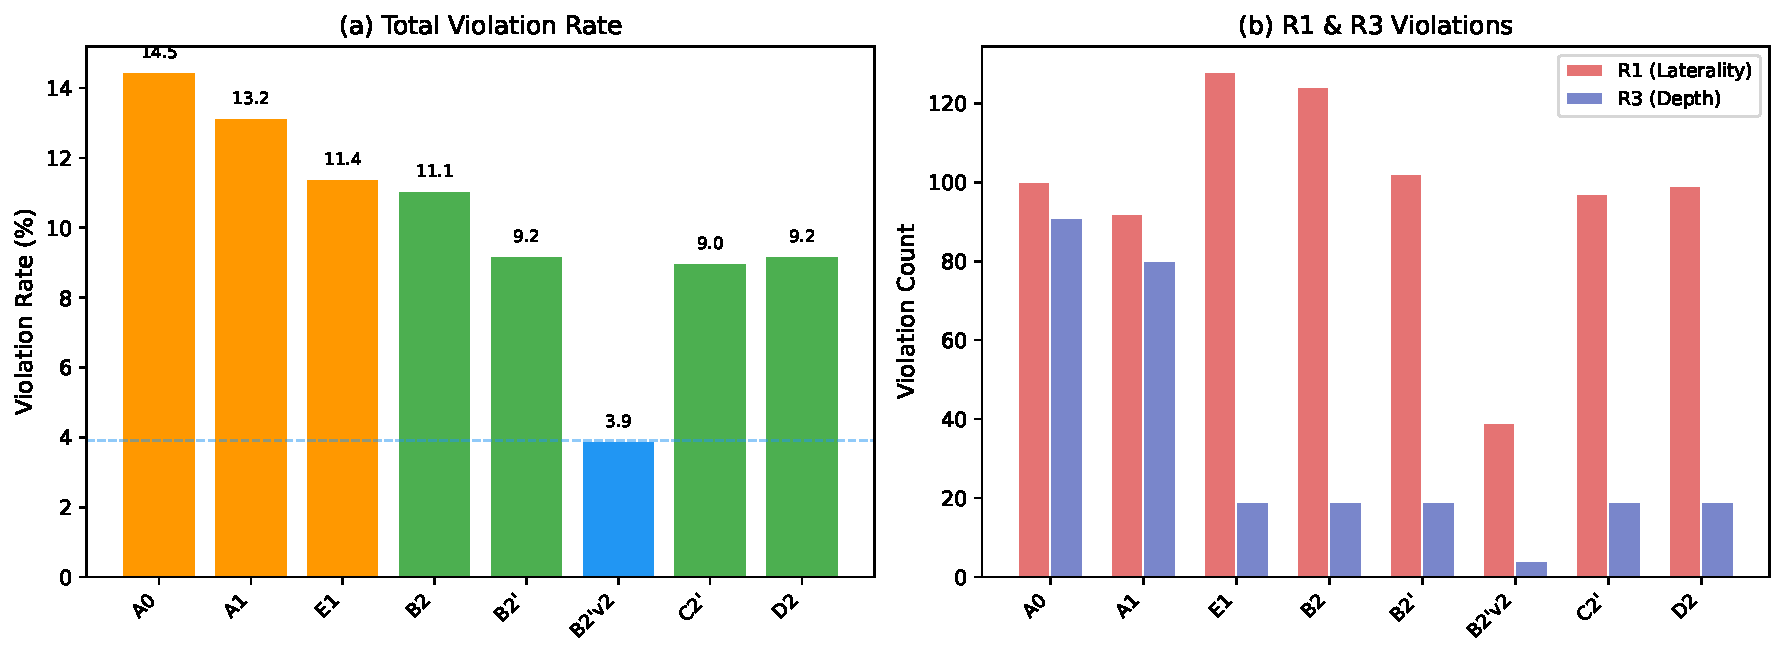
\includegraphics[width=\textwidth]{../outputs/paper_figures/fig1_waterfall.pdf}
\caption{Ablation chain progression. (a) Total violation rate (\%) showing the dramatic reduction at B2'v2 (Evidence Card v2). (b) Per-rule breakdown: R1 (laterality) and R3 (depth) violations. B2'v2 achieves the best balance with R1=39, R3=4.}
\label{fig:waterfall}
\end{figure}

\subsection{Sensitivity to $k$ (Tokens per Sentence)}

Figure~\ref{fig:budget_sweep} shows the effect of varying $k$ (tokens cited per sentence) on spatial consistency.
All configurations use E1 routing (spatial filter + semantic rerank) on 180 cases without LLM generation.

\begin{figure}[H]
\centering
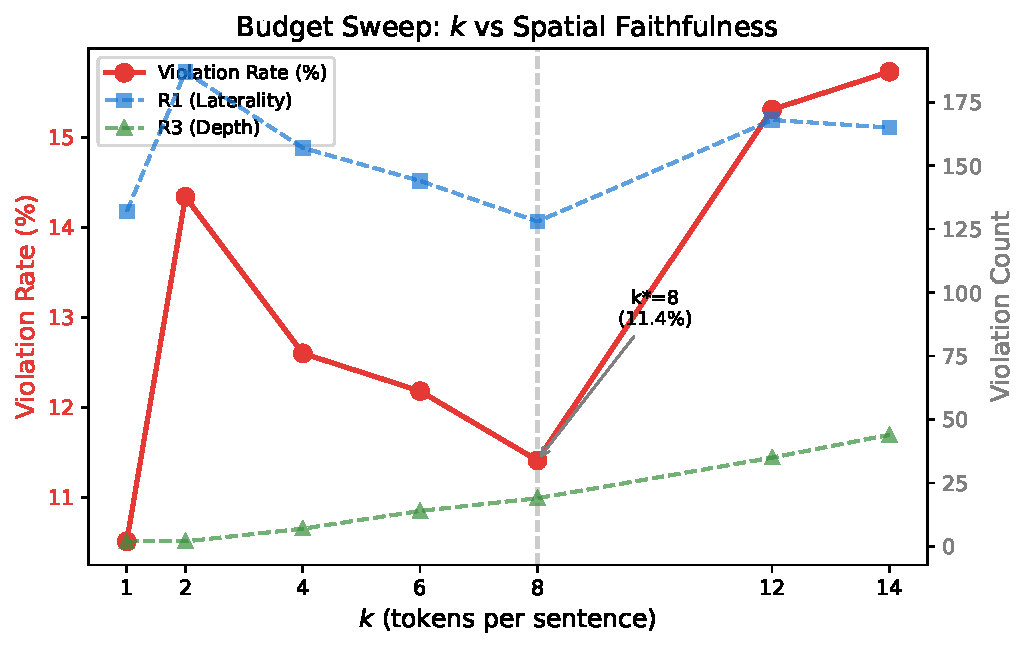
\includegraphics[width=0.75\textwidth]{../outputs/paper_figures/fig2_budget_sweep.pdf}
\caption{$k$ sensitivity: tokens per sentence vs spatial faithfulness.
The U-shaped violation rate curve reflects a trade-off: small $k$ causes laterality violations (R1, insufficient coverage), while large $k$ causes depth violations (R3, over-inclusion of coarse tokens).
Optimal $k^*{=}8$ minimizes total violation rate at 11.41\%.}
\label{fig:budget_sweep}
\end{figure}

\subsection{W\_proj Routing Strategy Ablation}

The three configurations in Table~\ref{tab:main_results} constitute a controlled ablation of the routing strategy:
\begin{itemize}[nosep]
\item \textbf{B2'v2 $\to$ E1:} Switching from anatomy-primary (IoU-dominant) to semantic-primary (trained $W_{\mathrm{proj}}$ + cosine rerank) trades R1 for R3.
\item \textbf{E1 $\to$ Hybrid E1:} Adding laterality hard filter to E1 --- no improvement (root cause: IoU-pass set empty for 98\% of R1 violations).
\end{itemize}

% ============================================================

\section{Counterfactual Sensitivity Analysis}
\label{sec:counterfactual}
% ============================================================

To validate that the verifier rules detect genuine spatial inconsistencies (rather than spurious patterns), we apply controlled perturbations to the 5K test set (3,979 sentences) and measure the change in violation rate.

\paragraph{Perturbations.}
\begin{itemize}[nosep]
\item \textbf{Paraphrase (control):} Synonym substitution in sentence text without changing spatial claims. Expected: no change in violation rate.
\item \textbf{Laterality flip:} Replace ``left'' $\leftrightarrow$ ``right'' in sentence text. Expected: R1 violations spike (tokens are on the wrong side).
\item \textbf{Presence flip:} Replace ``normal'' $\leftrightarrow$ ``abnormal'' for 50\% of eligible sentences. Expected: R6b cross-presence violations increase.
\end{itemize}

\paragraph{Results.}
Figure~\ref{fig:counterfactual} shows the results. All perturbations behave as expected:

\begin{figure}[H]
\centering
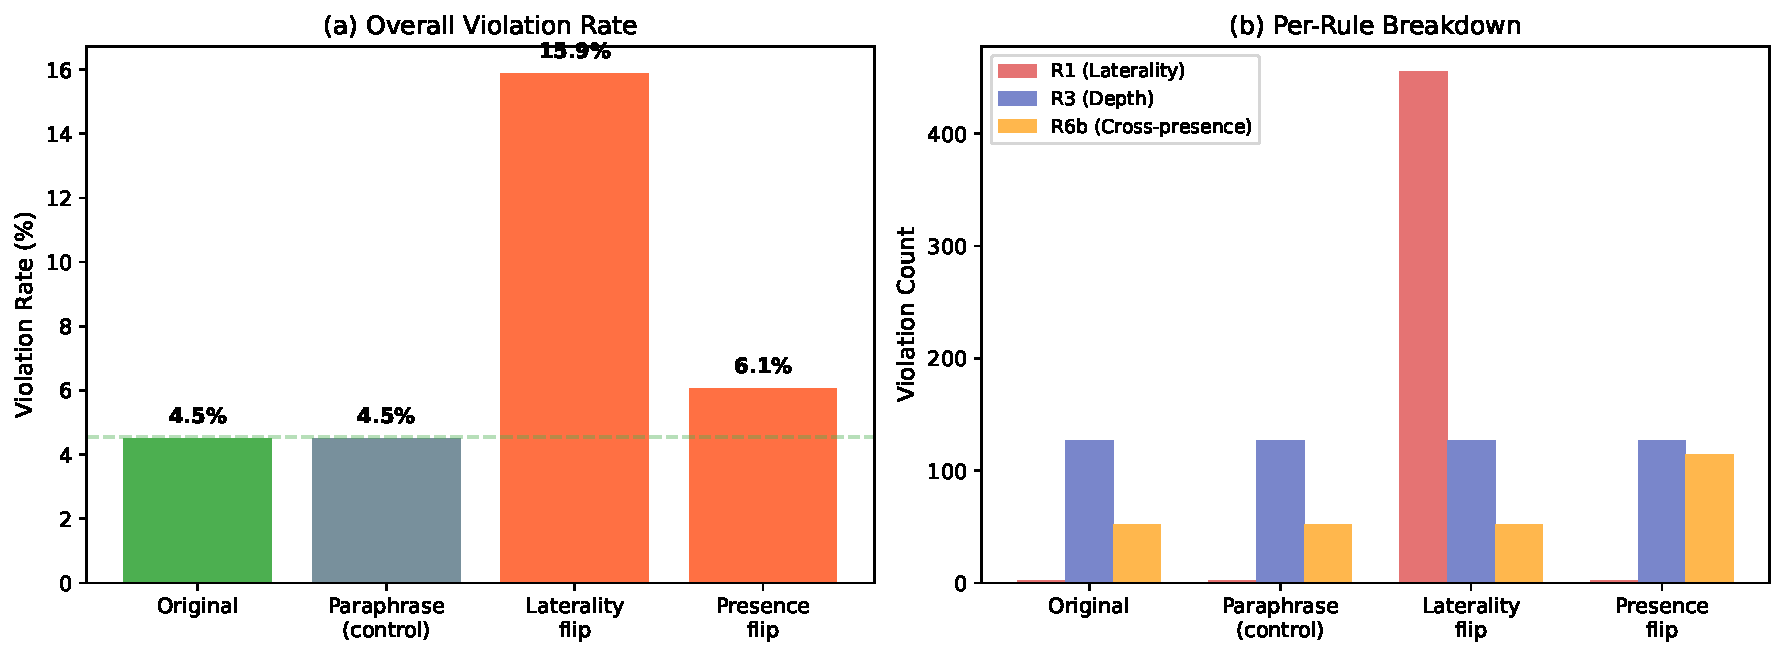
\includegraphics[width=\textwidth]{../outputs/paper_figures/fig3_counterfactual.pdf}
\caption{Counterfactual sensitivity analysis on 5K test set (3,979 sentences).
(a) Overall violation rate: paraphrase control is stable (4.5\% $\to$ 4.5\%), laterality flip spikes to 15.9\%, presence flip to 6.1\%.
(b) Per-rule breakdown: laterality flip increases R1 from 2 $\to$ 455 while R3 and R6b are unchanged; presence flip increases R6b from 52 $\to$ 114 while R1 and R3 are unchanged.
Each perturbation selectively triggers exactly the expected rule, confirming rule specificity.}
\label{fig:counterfactual}
\end{figure}

\begin{itemize}[nosep]
\item \textbf{Paraphrase stability:} Violation rate is identical (4.55\% $\to$ 4.55\%), confirming that our rules are robust to surface-level text variation.
\item \textbf{Laterality flip sensitivity:} R1 jumps from 2 $\to$ 455 ($+$453), violation rate 4.55\% $\to$ 15.93\%. R3 and R6b are unchanged, confirming that R1 specifically detects laterality mismatches.
\item \textbf{Presence flip sensitivity:} R6b jumps from 52 $\to$ 114 ($+$62), violation rate 4.55\% $\to$ 6.11\%. R1 and R3 are unchanged, confirming that R6b specifically detects cross-presence inconsistencies.
\end{itemize}


% ============================================================

\section{Qualitative Analysis}
\label{sec:qualitative}
% ============================================================

Figure~\ref{fig:qualitative} shows a representative example from the 5K test set (case \texttt{train\_10754\_c\_1}, CT-RATE).
Panel (a) shows the raw axial CT slice; panel (b) overlays the 8 routed tokens, which are spatially concentrated in the right lower lung; panel (c) displays the generated sentence with the Evidence Card metadata.

\begin{figure}[H]
\centering
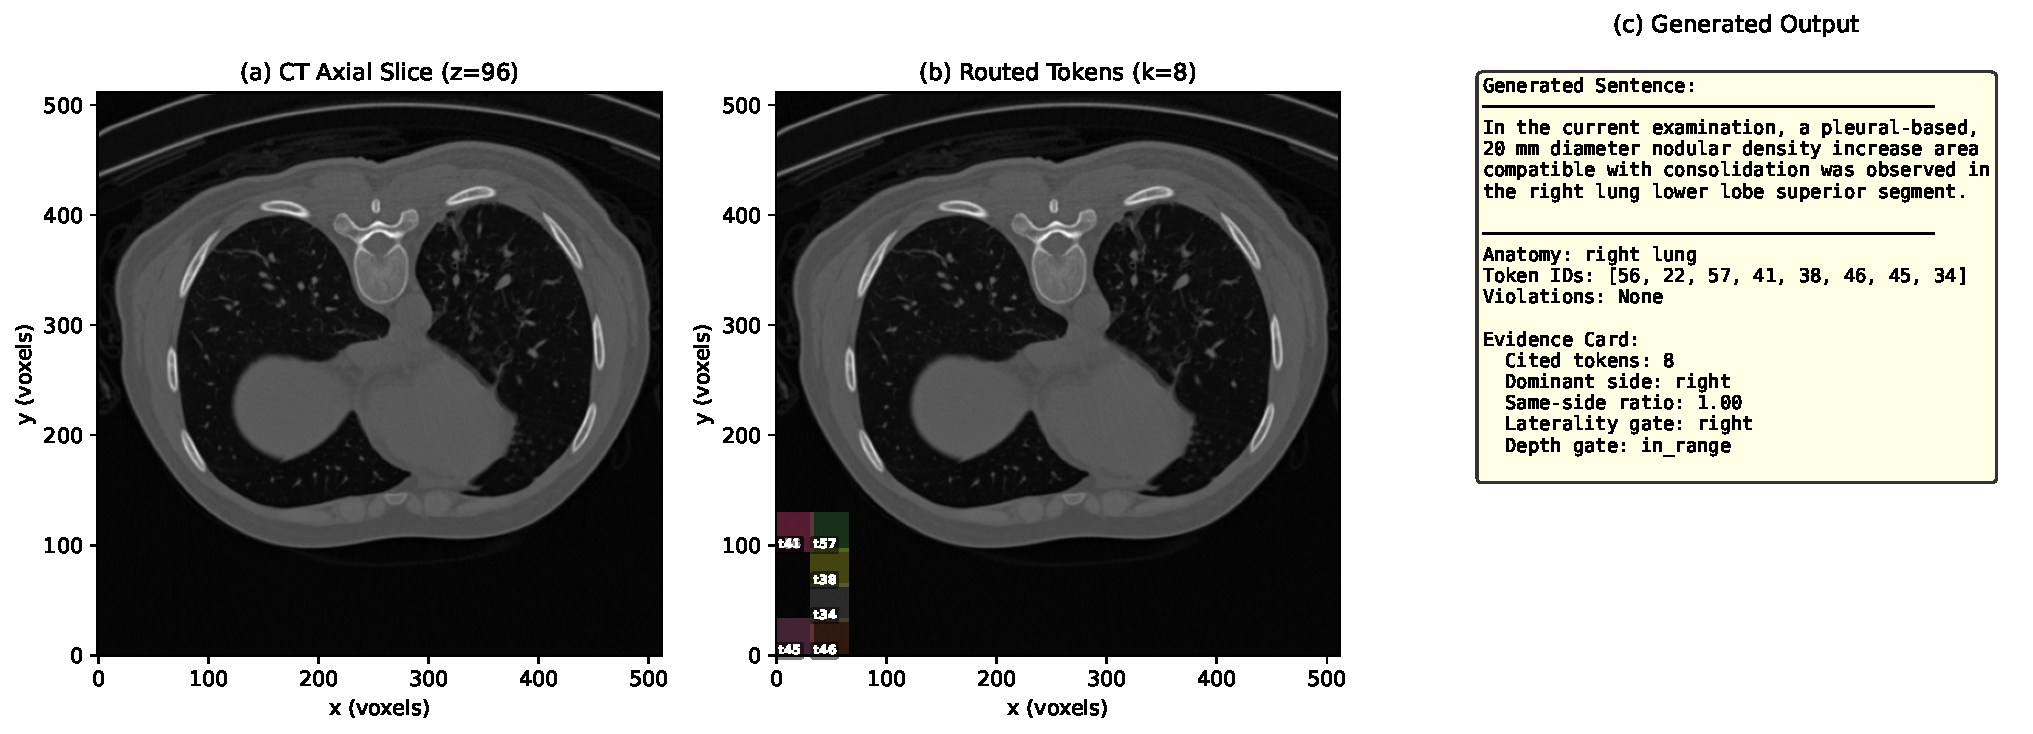
\includegraphics[width=\textwidth]{../outputs/paper_figures/fig4_qualitative.pdf}
\caption{Qualitative example. (a) CT axial slice at $z{=}96$. (b) Routed tokens ($k{=}8$) overlaid as colored bounding boxes, all localized in the right lower lung. (c) Generated sentence: ``a pleural-based, 20\,mm diameter nodular density increase area compatible with consolidation was observed in the right lung lower lobe superior segment.'' Evidence Card confirms: 8 cited tokens, dominant side = right, same-side ratio = 1.00, laterality gate = right, depth gate = in\_range. Zero violations.}
\label{fig:qualitative}
\end{figure}

% ============================================================

\section{Known Limitations}
\label{sec:limitations}
% ============================================================

\paragraph{L1: Re-route $\neq$ Re-split.}
Closed-loop re-routing can swap tokens within the fixed bank but cannot create new finer-grained tokens.
If failures are due to insufficient split depth, verifier-guided \emph{re-splitting} would be required (future work).

\paragraph{L2: Rule-based planning.}
Sentence planning is currently rule-based (regex extraction from reference text). This limits the system to settings where reference text is available (teacher-forced) or a fixed finding template is provided.

\paragraph{L3: Coarse anatomy atlas supervision.}
Atlas-based anatomy-to-bbox mapping is approximate (region/lobe-level, not segmentation-level).
Routing spatial priors and CT-RATE weak supervision are therefore coarse; RadGenome provides a stronger evaluation signal.

\paragraph{L4: Feature-space non-locality.}
Encode-then-split means cell features may be influenced by non-local receptive fields of the frozen encoder.

\paragraph{L5: Text serialization vs.\ visual prefix.}
By serializing evidence as text (rather than embedding visual tokens in the LLM hidden state), we lose the ability to leverage cross-attention between visual and textual representations. However, this design enables inspectability and works with any text-only LLM.

\paragraph{L6: Exposure bias from per-sentence autoregressive history.}
Per-sentence generation conditions on previously generated sentences; in open-loop inference, early errors may propagate to later sentences via the textual history.
We partially mitigate this by deriving routing queries from the plan (not from generated text).


% ============================================================
\appendix
\section{Stages 0--2 Detailed Specification (Token Bank Construction)}
\label{app:stage0-2}

\subsection{Stage 0: Artifact Pre-computation (Voxel Space)}

\begin{stagebox}{Stage 0 --- Artifact Risk Pre-computation}
\textcolor{inputcolor}{\textbf{Input:}} Raw CT volume $V \in \RR^{D\times H\times W}$.\\
\textcolor{outputcolor}{\textbf{Output:}} Per-cell artifact risk table $\{A_i\}$ for all initial coarse cells.
\end{stagebox}

\textbf{Definition.}
\begin{equation}
A_i = \clip\!\left(
    w_{\mathrm{snr}} \cdot \mathrm{norm}\!\left(\frac{\sigma_i}{|\mu_i|+\epsilon}\right)
    + w_{\mathrm{st}} \cdot \mathrm{norm}(\mathrm{streak}_i)
    + w_{\mathrm{out}} \cdot \mathrm{norm}(\mathrm{outlier}_i),\;
    0,\; 1
\right)
\label{eq:artifact}
\end{equation}
Computed in raw voxel space. Children recompute from raw volume after split.

\subsection{Stage 1: Encoding (One-shot, Frozen)}

\begin{stagebox}{Stage 1 --- Encoding}
\textcolor{inputcolor}{\textbf{Input:}} Raw CT volume $V$ (resized to $128^3$).\\
\textcolor{outputcolor}{\textbf{Output:}} Dense feature map $F \in \RR^{768 \times D' \times H' \times W'}$.
\end{stagebox}

Frozen SwinUNETR 3D encoder (feature\_size=48, pretrained on BTCV), one forward pass. The deepest encoder hidden state ($C{=}768$) is used. All subsequent operations on $F$.

\subsection{Stage 2: Adaptive Split (Core Module)}
\label{sec:split}

\begin{stagebox}{Stage 2 --- Adaptive Split}
\textcolor{inputcolor}{\textbf{Input:}} Feature map $F$; artifact table $\{A_i\}$ from Stage~0.\\
\textcolor{outputcolor}{\textbf{Output:}} Top-$B$ evidence tokens with features, bboxes, and scores.
\end{stagebox}

\subsubsection{Step 2.1: Initialization}
Octree at $d_0 = 2$ on $128^3$ volume $\Rightarrow$ $4^3 = 64$ coarse leaves.

\subsubsection{Step 2.2: Per-cell Scoring}

\paragraph{(a) Artifact Soft Gate.}
\begin{equation}
g_i = \sigmoid\!\big(-k\,(A_i - \tau_A)\big)
\label{eq:softgate}
\end{equation}
Default: $k=15$, $\tau_A=0.85$.

\paragraph{(b) Uncertainty Branch $H_i$.}
\begin{equation}
H_i = w_e \cdot \mathrm{norm}(H_i^{\mathrm{ent}}) + w_v \cdot \mathrm{norm}(H_i^{\mathrm{var}}) + w_b \cdot \mathrm{norm}(B_i)
\end{equation}
with $w_e{+}w_v{+}w_b{=}1$, default $(0.5, 0.3, 0.2)$.

\paragraph{(c) Semantic Prior $P_i$.}
\begin{equation}
P_i = \sigmoid\!\big(\mathrm{mean}(\lVert F\rVert_{\Omega_i}) - \theta_p\big)
\end{equation}

\paragraph{(d) Final Score.}
\begin{equation}
\boxed{S_i = g_i \cdot \Big(\lambda_h \, q(H_i) + \lambda_p \, q(P_i)\Big)}
\label{eq:score}
\end{equation}
$\lambda_h + \lambda_p = 1$. Default: $\lambda_h = 0.6$, $\lambda_p = 0.4$.

\subsubsection{Step 2.5: Token Export with Boundary Caching}

\paragraph{Overlap margin.}
Each exported token's feature pooling region is expanded by:
\begin{equation}
\Omega_i^{\mathrm{export}} = \mathrm{expand}(\Omega_i, \delta), \quad \delta = 0.125 \times \mathrm{cell\_size}_i
\end{equation}

\paragraph{Boundary feature caching.}
\begin{equation}
\mathbf{b}_i = \frac{1}{|\mathcal{N}(i)|} \sum_{j \in \mathcal{N}(i)} \mathbf{f}_j
\label{eq:boundary_cache}
\end{equation}
\begin{equation}
\mathbf{f}_i^{\mathrm{export}} = (1 - \beta)\,\mathbf{f}_i + \beta\,\mathbf{b}_i, \quad \beta = 0.1.
\label{eq:boundary_blend}
\end{equation}

% ============================================================

\section{Mathematical Appendix}
% ============================================================

\subsection{Routing Score}

\paragraph{Text query encoding.}
\begin{equation}
\mathbf{q}_s = \frac{\mathrm{TextEnc}(s)}{\lVert \mathrm{TextEnc}(s) \rVert_2} \in \RR^{384}
\end{equation}

\paragraph{Visual token projection (Eq.~\ref{eq:projection}).}
\begin{equation}
\mathbf{v}_i = \frac{W_{\mathrm{proj}} \, \mathbf{f}_i}{\lVert W_{\mathrm{proj}} \, \mathbf{f}_i\rVert_2}, \quad W_{\mathrm{proj}} \in \RR^{384 \times 768}
\end{equation}

\paragraph{Cosine routing score (Eq.~\ref{eq:routing_score}).}
\begin{equation}
r_i^{(s)} = \mathbf{q}_s^\top \mathbf{v}_i \in [-1, 1]
\end{equation}

\paragraph{Spatial augmentation.}

Standard mode (Eq.~\ref{eq:spatial_routing}):
\begin{equation}
\hat{r}_i^{(s)} = r_i^{(s)} + \lambda_{\mathrm{spatial}} \cdot \mathrm{IoU}(\mathrm{bbox}_i, \mathrm{bbox}_{\mathrm{anatomy}}^{(s)})
\end{equation}

Anatomy-primary mode (Eq.~\ref{eq:anatomy_primary}, used in B2'v2):
\begin{equation}
\hat{r}_i^{(s)} = \mathrm{IoU}(\mathrm{bbox}_i, \mathrm{bbox}_{\mathrm{anatomy}}^{(s)}) + \epsilon \cdot r_i^{(s)}, \quad \epsilon = 0.05
\end{equation}

\subsection{InfoNCE Training Objective (Eq.~\ref{eq:infonce})}

Given batch $\{(\mathbf{q}_n, \bar{\mathbf{f}}_n^{+})\}_{n=1}^N$ where $\bar{\mathbf{f}}_n^{+} = \frac{1}{k}\sum_{j \in E_n} \mathbf{f}_j$ (mean of cited tokens):
\begin{equation}
\mathbf{p}_n = \frac{W_{\mathrm{proj}} \bar{\mathbf{f}}_n^{+}}{\lVert W_{\mathrm{proj}} \bar{\mathbf{f}}_n^{+} \rVert_2}, \quad
\mathcal{L} = -\frac{1}{N} \sum_{n=1}^{N} \log \frac{\exp(\hat{\mathbf{q}}_n^\top \mathbf{p}_n / \tau)}{\sum_{m=1}^{N} \exp(\hat{\mathbf{q}}_n^\top \mathbf{p}_m / \tau)}
\end{equation}
Positives: mean features of tokens cited by anatomy-primary routing (bootstrap supervision).
Negatives: in-batch query--projection pairs from other sentences.

\subsection{Log-Smooth Re-routing Penalty (Eq.~\ref{eq:log_smooth})}
\begin{equation}
r_i' = r_i - \gamma \cdot \ln(1 + \mathrm{sev}_i), \quad \gamma = 2.0
\end{equation}

\subsection{Stability and Statistical Protocol}
\begin{itemize}[nosep]
    \item Patient-level paired bootstrap CI (95\%, $R{=}5000$ resamples), Holm step-down correction.
    \item Verifier pass rate reported as both raw and judge-confirmed.
\end{itemize}

\end{document}
